\documentclass [11pt, a4wide, twoside]{article}

\usepackage{times}
\usepackage{epsfig}
\usepackage{ifthen}
\usepackage{xspace}
\usepackage{fancyhdr}
\usepackage[colorlinks = true,linkcolor = black,urlcolor  = blue,citecolor = black,anchorcolor = black]{hyperref}
\usepackage{verbatim}
\usepackage{amsmath}
\usepackage{graphicx}

\usepackage{listings}
\usepackage{color}
%\usepackage{enumitem}

\definecolor{dkgreen}{rgb}{0,0.6,0}
\definecolor{gray}{rgb}{0.5,0.5,0.5}
\definecolor{mauve}{rgb}{0.58,0,0.82}

\lstset{frame=tb,
language=Java,
aboveskip=3mm,
belowskip=3mm,
showstringspaces=false,
columns=flexible,
basicstyle={\small\ttfamily},
numbers=none,
numberstyle=\tiny\color{gray},
keywordstyle=\color{blue},
commentstyle=\color{dkgreen},
stringstyle=\color{mauve},
breaklines=true,
breakatwhitespace=true
tabsize=3
}

\newboolean{showsolution}
\setboolean{showsolution}{true} 

% \newlist{todolist}{itemize}{2}
% \setlist[todolist]{label=$\square$}
% \usepackage{pifont}
% \newcommand{\cmark}{\ding{51}}%
% \newcommand{\xmark}{\ding{55}}%
% \newcommand{\done}{\rlap{$\square$}{\raisebox{2pt}{\large\hspace{1pt}\cmark}}%
% \hspace{-2.5pt}}
% \newcommand{\wontfix}{\rlap{$\square$}{\large\hspace{1pt}\xmark}}


% \usepackage{times}
\usepackage{epsfig}
\usepackage{ifthen}
\usepackage{xspace}
\usepackage{fancyhdr}
\usepackage{amsthm}
\usepackage{hyperref}



%layout
\topmargin      -5.0mm
\oddsidemargin  6.0mm
\evensidemargin -6.0mm
\textheight     215.5mm
\textwidth      160.0mm
\parindent      1.0em
\headsep        10.3mm
\headheight     12pt
\lineskip       1pt
\normallineskip 1pt

\newtheorem{mydef}{Definition}


%header
\lhead{Software Modeling and Analysis \\ 2016}

\rhead{Prof. Oscar Nierstrasz, Mohammad Ghafari, Nevena Milojkovi\'{c} and Yuriy Tymchuk}

\lfoot{page \thepage}
\rfoot{\today}
\cfoot{}

\renewcommand{\headrulewidth}{0.1pt}
\renewcommand{\footrulewidth}{0.1pt}

%enumeration
\newenvironment{myitemize}{%
     \begin{itemize}
     \setlength{\itemsep}{0cm}}
     {\end{itemize}}

\newenvironment{myenumerate}{%
     \begin{enumerate} \setlength{\itemsep}{0cm}}
     {\end{enumerate}}


%solution
\ifthenelse{\boolean{showsolution}}
   {  \newcommand{\solution}[1]{
   	\noindent\underline{\textbf{Answer:}}\\[2mm]
   	 \textsl{#1}
	 \vspace{10pt}
	 \normalsize
	}
  }
  {  \newcommand{\solution}[1]{} }


\pagestyle{fancy}

% ============================================================
% Markup macros for proof-reading
\usepackage{ifthen}
\usepackage[normalem]{ulem} % for \sout
\usepackage{xcolor}
\newcommand{\ra}{$\rightarrow$}
\newboolean{showedits}
\setboolean{showedits}{true} % toggle to show or hide edits
\ifthenelse{\boolean{showedits}}
{
	\newcommand{\ugh}[1]{\textcolor{red}{\uwave{#1}}} % please rephrase
	\newcommand{\ins}[1]{\textcolor{blue}{\uline{#1}}} % please insert
	\newcommand{\del}[1]{\textcolor{red}{\sout{#1}}} % please delete
	\newcommand{\chg}[2]{\textcolor{red}{\sout{#1}}{\ra}\textcolor{blue}{\uline{#2}}} % please change
}{
	\newcommand{\ugh}[1]{#1} % please rephrase
	\newcommand{\ins}[1]{#1} % please insert
	\newcommand{\del}[1]{} % please delete
	\newcommand{\chg}[2]{#2}
}
% ============================================================
% Put edit comments in a really ugly standout display
%\usepackage{ifthen}
\usepackage{amssymb}
\newboolean{showcomments}
\setboolean{showcomments}{true}
%\setboolean{showcomments}{false}
\newcommand{\id}[1]{$-$Id: scgPaper.tex 32478 2010-04-29 09:11:32Z oscar $-$}
\newcommand{\yellowbox}[1]{\fcolorbox{gray}{yellow}{\bfseries\sffamily\scriptsize#1}}
\newcommand{\triangles}[1]{{\sf\small$\blacktriangleright$\textit{#1}$\blacktriangleleft$}}
\ifthenelse{\boolean{showcomments}}
%{\newcommand{\nb}[2]{{\yellowbox{#1}\triangles{#2}}}
{\newcommand{\nbc}[3]{
 {\colorbox{#3}{\bfseries\sffamily\scriptsize\textcolor{white}{#1}}}
 {\textcolor{#3}{\sf\small$\blacktriangleright$\textit{#2}$\blacktriangleleft$}}}
 \newcommand{\version}{\emph{\scriptsize\id}}}
{\newcommand{\nbc}[3]{}
 \renewcommand{\ugh}[1]{#1} % please rephrase
 \renewcommand{\ins}[1]{#1} % please insert
 \renewcommand{\del}[1]{} % please delete
 \renewcommand{\chg}[2]{#2} % please change
 \newcommand{\version}{}}
\newcommand{\nb}[2]{\nbc{#1}{#2}{orange}}
\newcommand{\here}{\yellowbox{$\Rightarrow$ CONTINUE HERE $\Leftarrow$}}
\newcommand\rev[2]{\nb{TODO (rev #1)}{#2}} % reviewer comments
\newcommand\fix[1]{\nb{FIX}{#1}}
\newcommand\todo[1]{\nb{TO DO}{#1}}
\newcommand\on[1]{\nbc{ON}{#1}{red}} % add more author macros here
%\newcommand\XXX[1]{\nbc{XXX}{#1}{blue}}
%\newcommand\XXX[1]{\nbc{XXX}{#1}{brown}}
%\newcommand\XXX[1]{\nbc{XXX}{#1}{cyan}}
%\newcommand\XXX[1]{\nbc{XXX}{#1}{darkgray}}
%\newcommand\XXX[1]{\nbc{XXX}{#1}{gray}}
%\newcommand\XXX[1]{\nbc{XXX}{#1}{magenta}}
%\newcommand\XXX[1]{\nbc{XXX}{#1}{olive}}
%\newcommand\XXX[1]{\nbc{XXX}{#1}{orange}}
%\newcommand\XXX[1]{\nbc{XXX}{#1}{purple}}
%\newcommand\XXX[1]{\nbc{XXX}{#1}{red}}
%\newcommand\XXX[1]{\nbc{XXX}{#1}{teal}}
%\newcommand\XXX[1]{\nbc{XXX}{#1}{violet}}
%=============================================================
% ST80 listings macros
% Adapted from Squeak by Example book
%=============================================================
% If you want >>> appearing as right guillemet, you need these two lines:
%\usepackage[T1]{fontenc}
%\newcommand{\sep}{\mbox{>>}}
% Otherwise use this:
\newcommand{\sep}{\mbox{$\gg$}}
%=============================================================
%:\needlines{N} before code block to force page feed
\usepackage{needspace}
\newcommand{\needlines}[1]{\Needspace{#1\baselineskip}}
%=============================================================
%:Listings package configuration for ST80
\usepackage[english]{babel}
\usepackage{amssymb,textcomp}
\usepackage{listings}
% \usepackage[usenames,dvipsnames]{color}
% \usepackage[usenames]{color}
% \definecolor{source}{gray}{0.95}
\lstdefinelanguage{Smalltalk}{
%  morekeywords={self,super,true,false,nil,thisContext}, % This is overkill
  morestring=[d]',
  morecomment=[s]{"}{"},
  alsoletter={\#:},
  escapechar={!},
  literate=
    {BANG}{!}1
    {UNDERSCORE}{\_}1
    {\\st}{Smalltalk}9 % convenience -- in case \st occurs in code
    % {'}{{\textquotesingle}}1 % replaced by upquote=true in \lstset
    {_}{{$\leftarrow$}}1
    {>>>}{{\sep}}1
    {^}{{$\uparrow$}}1
    {~}{{$\sim$}}1
    {-}{{\sf -\hspace{-0.13em}-}}1  % the goal is to make - the same width as +
    {+}{\raisebox{0.08ex}{+}}1		% and to raise + off the baseline to match -
    {-->}{{\quad$\longrightarrow$\quad}}3
	, % Don't forget the comma at the end!
  tabsize=4
}[keywords,comments,strings]

\definecolor{source}{gray}{0.95}

\lstset{language=Smalltalk,
	basicstyle=\sffamily,
	keywordstyle=\color{black}\bfseries,
	% stringstyle=\ttfamily, % Ugly! do we really want this? -- on
	mathescape=true,
	showstringspaces=false,
	keepspaces=true,
	breaklines=true,
	breakautoindent=true,
	backgroundcolor=\color{source},
	lineskip={-1pt}, % Ugly hack
	upquote=true, % straight quote; requires textcomp package
	columns=fullflexible} % no fixed width fonts
% In-line code (literal)
% Normally use this for all in-line code:
\newcommand{\ct}{\lstinline[mathescape=false,backgroundcolor=\color{white},basicstyle={\sffamily\upshape}]}
% In-line code (latex enabled)
% Use this only in special situations where \ct does not work
% (within section headings ...):
\newcommand{\lct}[1]{{\textsf{\textup{#1}}}}
% Code environments
\lstnewenvironment{code}{%
	\lstset{%
		% frame=lines,
		frame=single,
		framerule=0pt,
		mathescape=false
	}
}{}

% Useful to add a matching $ after code containing a $
% \def\ignoredollar#1{}
%=============================================================
\newcommand{\ie}{\emph{i.e.}\xspace}
\newcommand{\eg}{\emph{e.g.}\xspace}
\newcommand{\etal}{\emph{et al.}\xspace}
% ============================================================

% \definecolor{mircolor}{rgb}{0.4,0.6,0.2}
% \newcommand\ml[1]{\nbc{ML}{#1}{mircolor}}
% \usepackage{wasysym}
% \newcommand\yesml[1]{\nbc{ML {\textcolor{yellow}\sun}}{#1}{mircolor}}

\usepackage{times}
\usepackage{epsfig}
\usepackage{ifthen}
\usepackage{xspace}
\usepackage{fancyhdr}
\usepackage{amsthm}
\usepackage{hyperref}



%layout
\topmargin      -5.0mm
\oddsidemargin  6.0mm
\evensidemargin -6.0mm
\textheight     215.5mm
\textwidth      160.0mm
\parindent      1.0em
\headsep        10.3mm
\headheight     12pt
\lineskip       1pt
\normallineskip 1pt

\newtheorem{mydef}{Definition}


%header
\lhead{Software Modeling and Analysis \\ 2016}

\rhead{Prof. Oscar Nierstrasz, Mohammad Ghafari, Nevena Milojkovi\'{c} and Yuriy Tymchuk}

\lfoot{page \thepage}
\rfoot{\today}
\cfoot{}

\renewcommand{\headrulewidth}{0.1pt}
\renewcommand{\footrulewidth}{0.1pt}

%enumeration
\newenvironment{myitemize}{%
     \begin{itemize}
     \setlength{\itemsep}{0cm}}
     {\end{itemize}}

\newenvironment{myenumerate}{%
     \begin{enumerate} \setlength{\itemsep}{0cm}}
     {\end{enumerate}}


%solution
\ifthenelse{\boolean{showsolution}}
   {  \newcommand{\solution}[1]{
   	\noindent\underline{\textbf{Answer:}}\\[2mm]
   	 \textsl{#1}
	 \vspace{10pt}
	 \normalsize
	}
  }
  {  \newcommand{\solution}[1]{} }


\pagestyle{fancy}

% ============================================================
% Markup macros for proof-reading
\usepackage{ifthen}
\usepackage[normalem]{ulem} % for \sout
\usepackage{xcolor}
\newcommand{\ra}{$\rightarrow$}
\newboolean{showedits}
\setboolean{showedits}{true} % toggle to show or hide edits
\ifthenelse{\boolean{showedits}}
{
	\newcommand{\ugh}[1]{\textcolor{red}{\uwave{#1}}} % please rephrase
	\newcommand{\ins}[1]{\textcolor{blue}{\uline{#1}}} % please insert
	\newcommand{\del}[1]{\textcolor{red}{\sout{#1}}} % please delete
	\newcommand{\chg}[2]{\textcolor{red}{\sout{#1}}{\ra}\textcolor{blue}{\uline{#2}}} % please change
}{
	\newcommand{\ugh}[1]{#1} % please rephrase
	\newcommand{\ins}[1]{#1} % please insert
	\newcommand{\del}[1]{} % please delete
	\newcommand{\chg}[2]{#2}
}
% ============================================================
% Put edit comments in a really ugly standout display
%\usepackage{ifthen}
\usepackage{amssymb}
\newboolean{showcomments}
\setboolean{showcomments}{true}
%\setboolean{showcomments}{false}
\newcommand{\id}[1]{$-$Id: scgPaper.tex 32478 2010-04-29 09:11:32Z oscar $-$}
\newcommand{\yellowbox}[1]{\fcolorbox{gray}{yellow}{\bfseries\sffamily\scriptsize#1}}
\newcommand{\triangles}[1]{{\sf\small$\blacktriangleright$\textit{#1}$\blacktriangleleft$}}
\ifthenelse{\boolean{showcomments}}
%{\newcommand{\nb}[2]{{\yellowbox{#1}\triangles{#2}}}
{\newcommand{\nbc}[3]{
 {\colorbox{#3}{\bfseries\sffamily\scriptsize\textcolor{white}{#1}}}
 {\textcolor{#3}{\sf\small$\blacktriangleright$\textit{#2}$\blacktriangleleft$}}}
 \newcommand{\version}{\emph{\scriptsize\id}}}
{\newcommand{\nbc}[3]{}
 \renewcommand{\ugh}[1]{#1} % please rephrase
 \renewcommand{\ins}[1]{#1} % please insert
 \renewcommand{\del}[1]{} % please delete
 \renewcommand{\chg}[2]{#2} % please change
 \newcommand{\version}{}}
\newcommand{\nb}[2]{\nbc{#1}{#2}{orange}}
\newcommand{\here}{\yellowbox{$\Rightarrow$ CONTINUE HERE $\Leftarrow$}}
\newcommand\rev[2]{\nb{TODO (rev #1)}{#2}} % reviewer comments
\newcommand\fix[1]{\nb{FIX}{#1}}
\newcommand\todo[1]{\nb{TO DO}{#1}}
\newcommand\on[1]{\nbc{ON}{#1}{red}} % add more author macros here
%\newcommand\XXX[1]{\nbc{XXX}{#1}{blue}}
%\newcommand\XXX[1]{\nbc{XXX}{#1}{brown}}
%\newcommand\XXX[1]{\nbc{XXX}{#1}{cyan}}
%\newcommand\XXX[1]{\nbc{XXX}{#1}{darkgray}}
%\newcommand\XXX[1]{\nbc{XXX}{#1}{gray}}
%\newcommand\XXX[1]{\nbc{XXX}{#1}{magenta}}
%\newcommand\XXX[1]{\nbc{XXX}{#1}{olive}}
%\newcommand\XXX[1]{\nbc{XXX}{#1}{orange}}
%\newcommand\XXX[1]{\nbc{XXX}{#1}{purple}}
%\newcommand\XXX[1]{\nbc{XXX}{#1}{red}}
%\newcommand\XXX[1]{\nbc{XXX}{#1}{teal}}
%\newcommand\XXX[1]{\nbc{XXX}{#1}{violet}}
%=============================================================
% ST80 listings macros
% Adapted from Squeak by Example book
%=============================================================
% If you want >>> appearing as right guillemet, you need these two lines:
%\usepackage[T1]{fontenc}
%\newcommand{\sep}{\mbox{>>}}
% Otherwise use this:
\newcommand{\sep}{\mbox{$\gg$}}
%=============================================================
%:\needlines{N} before code block to force page feed
\usepackage{needspace}
\newcommand{\needlines}[1]{\Needspace{#1\baselineskip}}
%=============================================================
%:Listings package configuration for ST80
\usepackage[english]{babel}
\usepackage{amssymb,textcomp}
\usepackage{listings}
% \usepackage[usenames,dvipsnames]{color}
% \usepackage[usenames]{color}
% \definecolor{source}{gray}{0.95}
\lstdefinelanguage{Smalltalk}{
%  morekeywords={self,super,true,false,nil,thisContext}, % This is overkill
  morestring=[d]',
  morecomment=[s]{"}{"},
  alsoletter={\#:},
  escapechar={!},
  literate=
    {BANG}{!}1
    {UNDERSCORE}{\_}1
    {\\st}{Smalltalk}9 % convenience -- in case \st occurs in code
    % {'}{{\textquotesingle}}1 % replaced by upquote=true in \lstset
    {_}{{$\leftarrow$}}1
    {>>>}{{\sep}}1
    {^}{{$\uparrow$}}1
    {~}{{$\sim$}}1
    {-}{{\sf -\hspace{-0.13em}-}}1  % the goal is to make - the same width as +
    {+}{\raisebox{0.08ex}{+}}1		% and to raise + off the baseline to match -
    {-->}{{\quad$\longrightarrow$\quad}}3
	, % Don't forget the comma at the end!
  tabsize=4
}[keywords,comments,strings]

\definecolor{source}{gray}{0.95}

\lstset{language=Smalltalk,
	basicstyle=\sffamily,
	keywordstyle=\color{black}\bfseries,
	% stringstyle=\ttfamily, % Ugly! do we really want this? -- on
	mathescape=true,
	showstringspaces=false,
	keepspaces=true,
	breaklines=true,
	breakautoindent=true,
	backgroundcolor=\color{source},
	lineskip={-1pt}, % Ugly hack
	upquote=true, % straight quote; requires textcomp package
	columns=fullflexible} % no fixed width fonts
% In-line code (literal)
% Normally use this for all in-line code:
\newcommand{\ct}{\lstinline[mathescape=false,backgroundcolor=\color{white},basicstyle={\sffamily\upshape}]}
% In-line code (latex enabled)
% Use this only in special situations where \ct does not work
% (within section headings ...):
\newcommand{\lct}[1]{{\textsf{\textup{#1}}}}
% Code environments
\lstnewenvironment{code}{%
	\lstset{%
		% frame=lines,
		frame=single,
		framerule=0pt,
		mathescape=false
	}
}{}

% Useful to add a matching $ after code containing a $
% \def\ignoredollar#1{}
%=============================================================
\newcommand{\ie}{\emph{i.e.}\xspace}
\newcommand{\eg}{\emph{e.g.}\xspace}
\newcommand{\etal}{\emph{et al.}\xspace}
% ============================================================


\begin{document}

\section*{\ifthenelse{\boolean{showsolution}}{\textcolor{red}{Solution}\\}{}Assignment 10 --- 18.11.2020 -- v1.2\\Dynamic Program Analysis}

\textcolor{red}{Please submit this exercise by email to \href{mailto:pascal.gadient@inf.unibe.ch}{pascal.gadient@inf.unibe.ch} \underline{before} 25 November 2020, 10:15am.\begin{center}\textbf{You must submit your code as editable text, i.e., use plain text file(s).}\end{center}}

\subsection*{Exercise 1: Theory (1 pt)}
\begin{enumerate}[a)]
\item Suppose you have an application and you want to test all code paths with dynamic analysis. Is this approach reasonable? Justify!
\solution{No, it is not reasonable, because every single code path must be triggered in the application which is particularly hard if external input is involved.}
\item Is monkey testing a dynamic analysis technique? Justify!
\solution{Yes, it is. Monkey testing is a technique where a user (or system) provides on the fly random inputs to the (running) application under test. At that time, the application is monitored to detect potential issues.}
\end{enumerate}

\subsection*{Exercise 2: Contracts (3 pts)}
In this exercise, we use the syntax and features from \emph{jContracts} available~\href{http://jcontracts.sourceforge.net/}{here}.
Consider the Java code below.\\
\texttt{/**\\
\hspace*{0.225cm}* @pre number >= 100.0\\
\hspace*{0.225cm}* @post return == true\\
\hspace*{0.225cm}* @inv number < 0 || number >= 0\\
\hspace*{0.225cm}*/\\
public boolean add(int number) \{\\
\hspace*{0.5cm}if (number < 10) \{\\
\hspace*{1.0cm}this.number = this.number + number;\\        
\hspace*{1.0cm}return true;\\        
\hspace*{0.5cm}\} else \{\\
\hspace*{1.0cm}return false;\\
\hspace*{0.5cm}\}\\
\}}
\begin{enumerate}[a)]
\item Are the contracts for \texttt{add(int number)} valid, \ie exists a configuration that passes all three checks? If yes, which configuration succeeds? If no, what is the problem?
\solution{No, because the method is supposed to return true with an input value of at least 100. However, the method only returns true for numbers smaller than 10. This is a contradiction.}
\item Can the invariant contract be removed without any side effects? If yes, why do no side-effects occur? If no, which side-effects would occur?
\solution{Yes, this particular contract could be removed, because it does not enforce any meaningful constraints. That is, it only specifies that its value must reside within its value range.}
\item Suppose you have a Java method that calculates from a given number the number multiplied by itself as shown in the code below. Design a post contract that validates the result, \ie the contract must be violated whenever a result is wrong.\\\\
\texttt{public float square(int number) \{\\
\hspace*{0.5cm}return number * number;\\        
\}}\\\\
\solution{\texttt{@post Math.pow(number, 2) - return < 0.001}}
\end{enumerate}

\subsection*{Exercise 3: Profiling (3 pts)}
In this exercise, we use the Python programming language and a memory profiler package. If you do not already have Python installed please install it from~\href{https://www.python.org/downloads/}{here}. Next, you have to install the memory profiler package with the command \texttt{pip install -U memory\_profiler}. Please ensure that you execute that command with superuser access rights (use sudo on Linux and macOS, or right-click the shell executable and select "Run as administrator" on Windows). Next, please create a text file with the name \texttt{allocateMemory.py} that contains the Python code below.\\\\
\texttt{01\hspace*{1.0cm}@profile\\
02\hspace*{1.0cm}def getAllocatedMemory():\\
03\hspace*{1.0cm}\hspace*{0.5cm}a = [1] * (10 ** 6)\\
04\hspace*{1.0cm}\hspace*{0.5cm}b = [2] * (2 * 10 ** 7)\\
05\hspace*{1.0cm}\hspace*{0.5cm}del b\\
06\hspace*{1.0cm}\hspace*{0.5cm}return a\\
07\hspace*{1.0cm}\\
08\hspace*{1.0cm}if \_\_name\_\_ == \textquotesingle\_\_main\_\_\textquotesingle:\\
09\hspace*{1.0cm}\hspace*{0.5cm}getAllocatedMemory()\\
}\\
Finally, please execute \texttt{python -m memory\_profiler allocateMemory.py} and inspect the console output.

\begin{enumerate}[a)]
\item What is the return value of the method?
\solution{A list that contains the number ``1'' a million times.}
\item How much memory is consumed at most during the execution?
\solution{Around 96.5 MBytes. This number depends on various external factors such as operating system, Python version, Garbage collector state, etc.}
\item In which line is the most memory consumed during the execution of this method?
\solution{In line 4.}
\item What does the command \texttt{del b} do?
\solution{The command removes the variable name from the namespace. As a result, it cannot be referenced anymore and consequently it will be picked up by the garbage collector (GC). Afterwards, the GC can free its space.}
\item Is it mandatory to use the \texttt{del} command to free memory in Python?
\solution{No. Python has a built-in garbage collector that frees memory of objects that are not referenced anymore.}
\item How could you improve the memory consumption without changing the return value of the method?
\solution{You could safely remove line 4 (and 5). Both statements do not contribute to the return value.}
\end{enumerate}

\newpage

\subsection*{Exercise 4: Code coverage (3 pts)}
In this exercise, we will have a look at the output of \emph{gcov}, a dynamic analysis code coverage reporting tool that comes with~\href{https://gcc.gnu.org/}{\emph{GCC}}. To obtain code coverage data from an application with \emph{gcov}, you need to (re)compile its source code with a compiler from \emph{GCC}, and you have to set additional parameters so that the compiler injects on the fly code for collecting statistics during run time. In the next step, the newly generated binary must be executed. During the execution, the application itself logs statistics and stores them in a file. Finally, \emph{gcov} opens these generated files and presents them in a nice textual representation. Because the set up of \emph{GCC} can be cumbersome (especially on Windows machines) we already performed the outlined steps for you.\\\\
The generated output of \emph{gcov} shown below was generated for a simple Fibonacci application. When executed, the Fibonacci application asked the user to enter the number of iterations to perform.\\\\
You can find more details regarding the output format of \emph{gcov} in the corresponding man pages which you can find~\href{https://www.man7.org/linux/man-pages/man1/gcov.1.html}{here}.\\\\
\texttt{
\hspace*{0.925cm}-:\hspace*{0.74cm}0:\hspace*{0.75cm}Source:fibonacci.c\\
\hspace*{0.925cm}-:\hspace*{0.74cm}0:\hspace*{0.75cm}Graph:fibonacci.gcno\\
\hspace*{0.925cm}-:\hspace*{0.74cm}0:\hspace*{0.75cm}Data:fibonacci.gcda\\
\hspace*{0.925cm}-:\hspace*{0.74cm}0:\hspace*{0.75cm}Runs:1\\
\hspace*{0.925cm}-:\hspace*{0.74cm}1:\hspace*{0.75cm}\#include \textless stdio.h\textgreater\\
\hspace*{0.925cm}1:\hspace*{0.74cm}2:\hspace*{0.75cm}int main() \{\\
\hspace*{0.925cm}1:\hspace*{0.74cm}3:\hspace*{0.75cm}\hspace*{0.5cm}int i, n, t1 = 0, t2 = 1, nextTerm;\\
\hspace*{0.925cm}1:\hspace*{0.74cm}4:\hspace*{0.75cm}\hspace*{0.5cm}printf("Enter the number of iterations to perform: ");\\
\hspace*{0.925cm}1:\hspace*{0.74cm}5:\hspace*{0.75cm}\hspace*{0.5cm}scanf("\%d", \&n);\\
\hspace*{0.925cm}-:\hspace*{0.74cm}6:\\
\hspace*{0.925cm}1:\hspace*{0.74cm}7:\hspace*{0.75cm}\hspace*{0.5cm}if (n \textgreater~50) \{\\
\#\#\#\#\#:\hspace{0.74cm}8:\hspace*{0.75cm}\hspace*{1.0cm}printf("This will take some time, please be patient.\textbackslash n");\\
\hspace*{0.925cm}-:\hspace*{0.74cm}9:\hspace*{0.75cm}\hspace*{0.5cm}\}\\
\hspace*{0.925cm}-:\hspace*{0.5cm}10:\\
\hspace*{0.925cm}1:\hspace*{0.5cm}11:\hspace*{0.75cm}\hspace*{0.5cm}printf("Fibonacci series: ");\\
\hspace*{0.7cm}13:\hspace*{0.5cm}12:\hspace*{0.75cm}\hspace*{0.5cm}for (i = 1; i \textless= n; ++i) \{\\
\hspace*{0.7cm}12:\hspace*{0.5cm}13:\hspace*{0.75cm}\hspace*{1.0cm}printf("\%d, ", t1);\\
\hspace*{0.7cm}12:\hspace*{0.5cm}14:\hspace*{0.75cm}\hspace*{1.0cm}nextTerm = t1 + t2;\\
\hspace*{0.7cm}12:\hspace*{0.5cm}15:\hspace*{0.75cm}\hspace*{1.0cm}t1 = t2;\\
\hspace*{0.7cm}12:\hspace*{0.5cm}16:\hspace*{0.75cm}\hspace*{1.0cm}t2 = nextTerm;\\
\hspace*{0.925cm}-:\hspace*{0.5cm}17:\hspace*{0.75cm}\hspace*{0.5cm}\}\\
\hspace*{0.925cm}-:\hspace*{0.5cm}18:\\
\hspace*{0.925cm}1:\hspace*{0.5cm}19:\hspace*{0.75cm}\hspace*{0.5cm}return 0;\\
\hspace*{0.925cm}-:\hspace*{0.5cm}20:\hspace*{0.75cm}\}}\\

\newpage

\begin{enumerate}[a)]
\item How many times has the application been executed in order to collect code coverage data?
\solution{The application has been executed only once (see ``Runs:1'').}
\item How many lines have been executed?
\solution{12 lines have been executed.}
\item How many lines have \underline{not} been executed?
\solution{A single line was not executed.}
\item Which statement was executed more than any other statement?
\solution{The head of the for-loop in line 12. It was executed 13 times.}
\item Which fibonacci number has been provided by the user?
\solution{12. We can see that on the number of executions of the code block in the for-loop.}
\item What is a fundamental limitation of dynamic analyses? In other words, what is the problem with user input?
\solution{Dynamic analyses rely on the comprehensive execution of code. Unfortunately, all potentially possible user input would need to be entered into the application to reach every code path, which is impossible. This problem can already have an impact on projects as small as our toy example: we only executed the code once and entered the value 12. Thus, we did not execute the code in the condition that checks for values greater than 50.}
\end{enumerate}

\newpage

\subsection*{Exercise 5: Invariant detection (3 pts BONUS)}
In this exercise, we will work with an analysis output of Daikon. Daikon is open-source software and its documentation can be found~\href{http://plse.cs.washington.edu/daikon/download/doc/}{here}. Inspect the code below and answer the corresponding questions.\\

\begin{figure}[h]
\centering
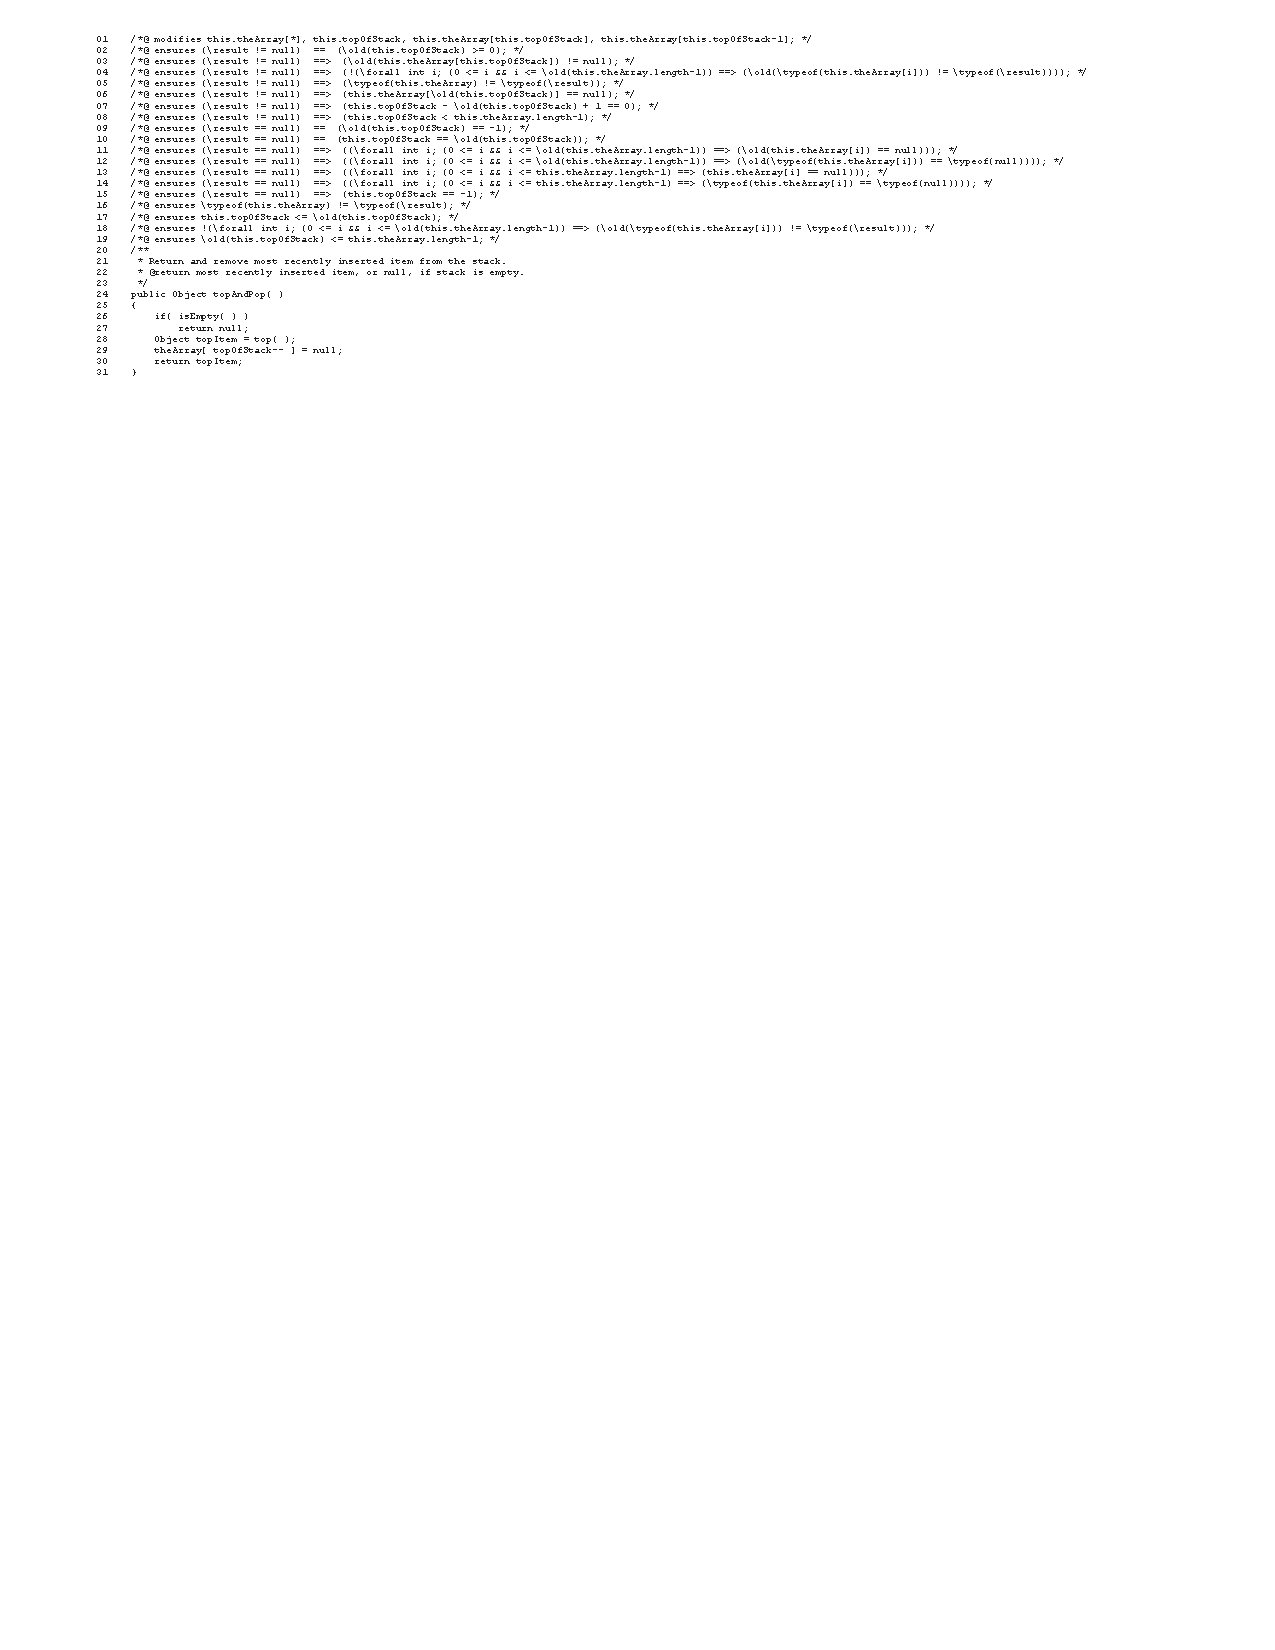
\includegraphics[scale=1.0,trim=1.9cm 22cm 2cm 1cm]{figures/Daikon.pdf}
\end{figure}

\begin{enumerate}[a)]
\item To which line in the Java code corresponds the postcondition in line 06?
\solution{Line 29.}
\item Why does the postcondition in line 02 use greater than or equal (\texttt{\textgreater=}), but not strict inequality (\texttt{\textgreater})?
\solution{Because \texttt{this.topOfStack == 0} is an acceptable scenario. It shows that the stack is empty and the method \texttt{topAndPop()} contains code to handle this situation (see lines 26 and 27); it would simply return \texttt{null}.}
\item What are the possible values for the variable \texttt{this.topOfStack} according to the relevant postconditions of \texttt{topAndPop()}? Please report for each relevant postcondition its line number and the value-related constraints.\\\\
\solution{\texttt{this.topOfStack} can only hold the value \texttt{-1} or a value within the range \\\texttt{[0; this.theArray.length - 1)}.\\\\
The relevant postconditions and value-related constraints are:\\
\footnotesize\texttt{02\hspace*{0.25cm}/*@ ensures (\textbackslash result != null)  ==  (\textbackslash old(this.topOfStack) \textgreater= 0); */\\
08\hspace*{0.25cm}/*@ ensures (\textbackslash result != null)  ==\textgreater~(this.topOfStack \textless~this.theArray.length-1); */\\
15\hspace*{0.25cm}/*@ ensures (\textbackslash result == null)  ==\textgreater~(this.topOfStack == -1); */}\normalsize}\\
\end{enumerate}

\end{document}
